\documentclass[1p]{elsarticle_modified}
%\bibliographystyle{elsarticle-num}

%\usepackage[colorlinks]{hyperref}
%\usepackage{abbrmath_seonhwa} %\Abb, \Ascr, \Acal ,\Abf, \Afrak
\usepackage{amsfonts}
\usepackage{amssymb}
\usepackage{amsmath}
\usepackage{amsthm}
\usepackage{scalefnt}
\usepackage{amsbsy}
\usepackage{kotex}
\usepackage{caption}
\usepackage{subfig}
\usepackage{color}
\usepackage{graphicx}
\usepackage{xcolor} %% white, black, red, green, blue, cyan, magenta, yellow
\usepackage{float}
\usepackage{setspace}
\usepackage{hyperref}

\usepackage{tikz}
\usetikzlibrary{arrows}

\usepackage{multirow}
\usepackage{array} % fixed length table
\usepackage{hhline}

%%%%%%%%%%%%%%%%%%%%%
\makeatletter
\renewcommand*\env@matrix[1][\arraystretch]{%
	\edef\arraystretch{#1}%
	\hskip -\arraycolsep
	\let\@ifnextchar\new@ifnextchar
	\array{*\c@MaxMatrixCols c}}
\makeatother %https://tex.stackexchange.com/questions/14071/how-can-i-increase-the-line-spacing-in-a-matrix
%%%%%%%%%%%%%%%

\usepackage[normalem]{ulem}

\newcommand{\msout}[1]{\ifmmode\text{\sout{\ensuremath{#1}}}\else\sout{#1}\fi}
%SOURCE: \msout is \stkout macro in https://tex.stackexchange.com/questions/20609/strikeout-in-math-mode

\newcommand{\cancel}[1]{
	\ifmmode
	{\color{red}\msout{#1}}
	\else
	{\color{red}\sout{#1}}
	\fi
}

\newcommand{\add}[1]{
	{\color{blue}\uwave{#1}}
}

\newcommand{\replace}[2]{
	\ifmmode
	{\color{red}\msout{#1}}{\color{blue}\uwave{#2}}
	\else
	{\color{red}\sout{#1}}{\color{blue}\uwave{#2}}
	\fi
}

\newcommand{\Sol}{\mathcal{S}} %segment
\newcommand{\D}{D} %diagram
\newcommand{\A}{\mathcal{A}} %arc


%%%%%%%%%%%%%%%%%%%%%%%%%%%%%5 test

\def\sl{\operatorname{\textup{SL}}(2,\Cbb)}
\def\psl{\operatorname{\textup{PSL}}(2,\Cbb)}
\def\quan{\mkern 1mu \triangleright \mkern 1mu}

\theoremstyle{definition}
\newtheorem{thm}{Theorem}[section]
\newtheorem{prop}[thm]{Proposition}
\newtheorem{lem}[thm]{Lemma}
\newtheorem{ques}[thm]{Question}
\newtheorem{cor}[thm]{Corollary}
\newtheorem{defn}[thm]{Definition}
\newtheorem{exam}[thm]{Example}
\newtheorem{rmk}[thm]{Remark}
\newtheorem{alg}[thm]{Algorithm}

\newcommand{\I}{\sqrt{-1}}
\begin{document}

%\begin{frontmatter}
%
%\title{Boundary parabolic representations of knots up to 8 crossings}
%
%%% Group authors per affiliation:
%\author{Yunhi Cho} 
%\address{Department of Mathematics, University of Seoul, Seoul, Korea}
%\ead{yhcho@uos.ac.kr}
%
%
%\author{Seonhwa Kim} %\fnref{s_kim}}
%\address{Center for Geometry and Physics, Institute for Basic Science, Pohang, 37673, Korea}
%\ead{ryeona17@ibs.re.kr}
%
%\author{Hyuk Kim}
%\address{Department of Mathematical Sciences, Seoul National University, Seoul 08826, Korea}
%\ead{hyukkim@snu.ac.kr}
%
%\author{Seokbeom Yoon}
%\address{Department of Mathematical Sciences, Seoul National University, Seoul, 08826,  Korea}
%\ead{sbyoon15@snu.ac.kr}
%
%\begin{abstract}
%We find all boundary parabolic representation of knots up to 8 crossings.
%
%\end{abstract}
%\begin{keyword}
%    \MSC[2010] 57M25 
%\end{keyword}
%
%\end{frontmatter}

%\linenumbers
%\tableofcontents
%
\newcommand\colored[1]{\textcolor{white}{\rule[-0.35ex]{0.8em}{1.4ex}}\kern-0.8em\color{red} #1}%
%\newcommand\colored[1]{\textcolor{white}{ #1}\kern-2.17ex	\textcolor{white}{ #1}\kern-1.81ex	\textcolor{white}{ #1}\kern-2.15ex\color{red}#1	}

{\Large $\underline{11a_{145}~(K11a_{145})}$}

\setlength{\tabcolsep}{10pt}
\renewcommand{\arraystretch}{1.6}
\vspace{1cm}\begin{tabular}{m{100pt}>{\centering\arraybackslash}m{274pt}}
\multirow{5}{120pt}{
	\centering
	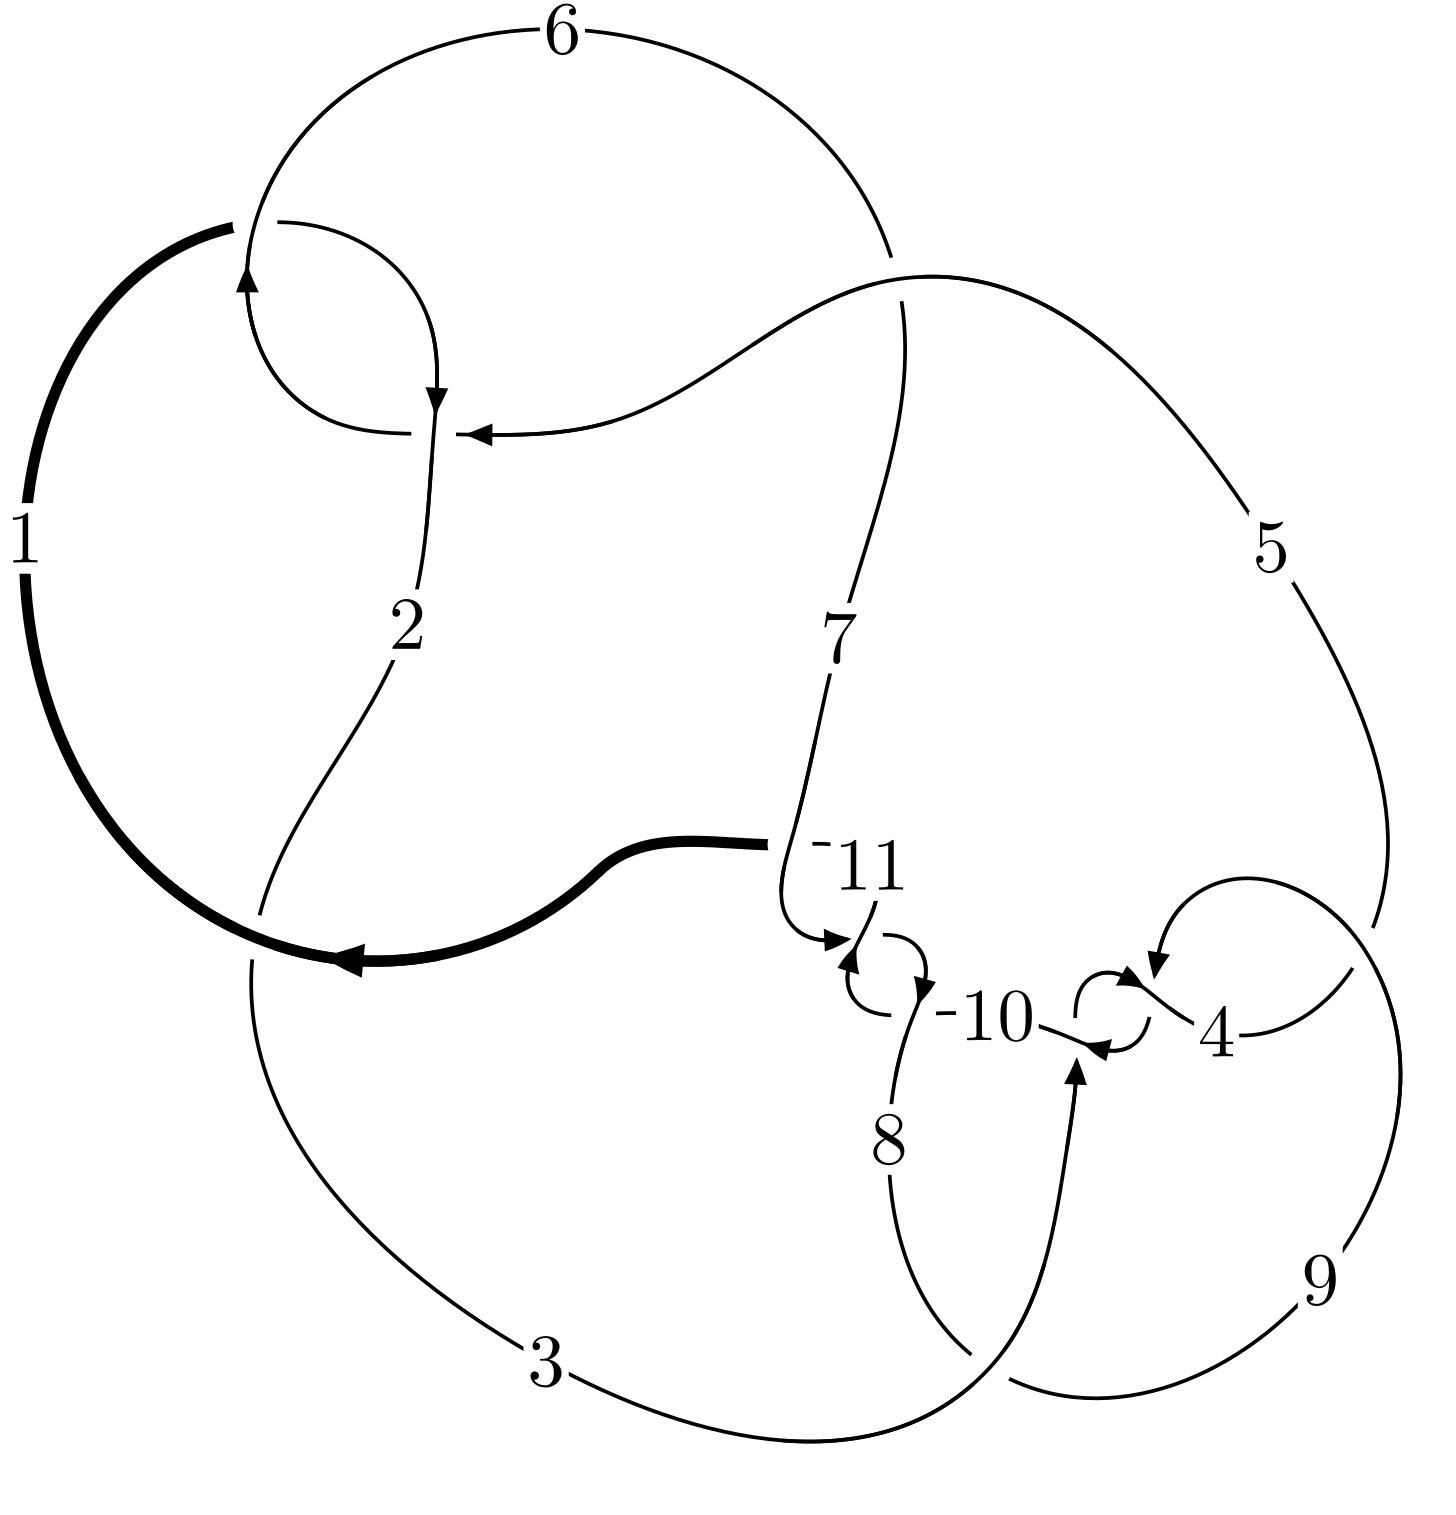
\includegraphics[width=112pt]{../../../GIT/diagram.site/Diagrams/png/394_11a_145.png}\\
\ \ \ A knot diagram\footnotemark}&
\allowdisplaybreaks
\textbf{Linearized knot diagam} \\
\cline{2-2}
 &
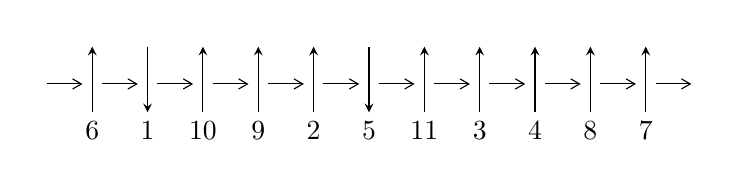
\begin{tikzpicture}[x=20pt, y=17pt]
	% nodes
	\node (C0) at (0, 0) {};
	\node (C1) at (1, 0) {};
	\node (C1U) at (1, +1) {};
	\node (C1D) at (1, -1) {6};

	\node (C2) at (2, 0) {};
	\node (C2U) at (2, +1) {};
	\node (C2D) at (2, -1) {1};

	\node (C3) at (3, 0) {};
	\node (C3U) at (3, +1) {};
	\node (C3D) at (3, -1) {10};

	\node (C4) at (4, 0) {};
	\node (C4U) at (4, +1) {};
	\node (C4D) at (4, -1) {9};

	\node (C5) at (5, 0) {};
	\node (C5U) at (5, +1) {};
	\node (C5D) at (5, -1) {2};

	\node (C6) at (6, 0) {};
	\node (C6U) at (6, +1) {};
	\node (C6D) at (6, -1) {5};

	\node (C7) at (7, 0) {};
	\node (C7U) at (7, +1) {};
	\node (C7D) at (7, -1) {11};

	\node (C8) at (8, 0) {};
	\node (C8U) at (8, +1) {};
	\node (C8D) at (8, -1) {3};

	\node (C9) at (9, 0) {};
	\node (C9U) at (9, +1) {};
	\node (C9D) at (9, -1) {4};

	\node (C10) at (10, 0) {};
	\node (C10U) at (10, +1) {};
	\node (C10D) at (10, -1) {8};

	\node (C11) at (11, 0) {};
	\node (C11U) at (11, +1) {};
	\node (C11D) at (11, -1) {7};
	\node (C12) at (12, 0) {};

	% arrows
	\draw[->,>={angle 60}]
	(C0) edge (C1) (C1) edge (C2) (C2) edge (C3) (C3) edge (C4) (C4) edge (C5) (C5) edge (C6) (C6) edge (C7) (C7) edge (C8) (C8) edge (C9) (C9) edge (C10) (C10) edge (C11) (C11) edge (C12) ;	\draw[->,>=stealth]
	(C1D) edge (C1U) (C2U) edge (C2D) (C3D) edge (C3U) (C4D) edge (C4U) (C5D) edge (C5U) (C6U) edge (C6D) (C7D) edge (C7U) (C8D) edge (C8U) (C9D) edge (C9U) (C10D) edge (C10U) (C11D) edge (C11U) ;
	\end{tikzpicture} \\
\hhline{~~} \\& 
\textbf{Solving Sequence} \\ \cline{2-2} 
 &
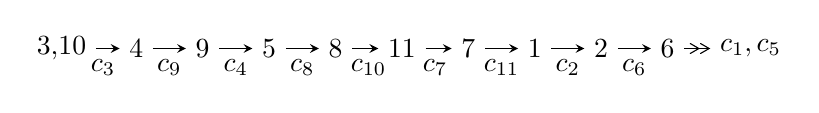
\begin{tikzpicture}[x=24pt, y=7pt]
	% node
	\node (A0) at (-1/8, 0) {3,10};
	\node (A1) at (1, 0) {4};
	\node (A2) at (2, 0) {9};
	\node (A3) at (3, 0) {5};
	\node (A4) at (4, 0) {8};
	\node (A5) at (5, 0) {11};
	\node (A6) at (6, 0) {7};
	\node (A7) at (7, 0) {1};
	\node (A8) at (8, 0) {2};
	\node (A9) at (9, 0) {6};
	\node (C1) at (1/2, -1) {$c_{3}$};
	\node (C2) at (3/2, -1) {$c_{9}$};
	\node (C3) at (5/2, -1) {$c_{4}$};
	\node (C4) at (7/2, -1) {$c_{8}$};
	\node (C5) at (9/2, -1) {$c_{10}$};
	\node (C6) at (11/2, -1) {$c_{7}$};
	\node (C7) at (13/2, -1) {$c_{11}$};
	\node (C8) at (15/2, -1) {$c_{2}$};
	\node (C9) at (17/2, -1) {$c_{6}$};
	\node (A10) at (41/4, 0) {$c_{1},c_{5}$};

	% edge
	\draw[->,>=stealth]	
	(A0) edge (A1) (A1) edge (A2) (A2) edge (A3) (A3) edge (A4) (A4) edge (A5) (A5) edge (A6) (A6) edge (A7) (A7) edge (A8) (A8) edge (A9) ;
	\draw[->>,>={angle 60}]	
	(A9) edge (A10);
\end{tikzpicture} \\ 

\end{tabular} \\

\footnotetext{
The image of knot diagram is generated by the software ``\textbf{Draw programme}" developed by Andrew Bartholomew(\url{http://www.layer8.co.uk/maths/draw/index.htm\#Running-draw}), where we modified some parts for our purpose(\url{https://github.com/CATsTAILs/LinksPainter}).
}\phantom \\ \newline 
\centering \textbf{Ideals for irreducible components\footnotemark of $X_{\text{par}}$} 
 
\begin{align*}
I^u_{1}&=\langle 
u^{41}+u^{40}+\cdots+u+1\rangle \\
\\
\end{align*}
\raggedright * 1 irreducible components of $\dim_{\mathbb{C}}=0$, with total 41 representations.\\
\footnotetext{All coefficients of polynomials are rational numbers. But the coefficients are sometimes approximated in decimal forms when there is not enough margin.}
\newpage
\renewcommand{\arraystretch}{1}
\centering \section*{I. $I^u_{1}= \langle u^{41}+u^{40}+\cdots+u+1 \rangle$}
\flushleft \textbf{(i) Arc colorings}\\
\begin{tabular}{m{7pt} m{180pt} m{7pt} m{180pt} }
\flushright $a_{3}=$&$\begin{pmatrix}1\\0\end{pmatrix}$ \\
\flushright $a_{10}=$&$\begin{pmatrix}0\\u\end{pmatrix}$ \\
\flushright $a_{4}=$&$\begin{pmatrix}1\\- u^2\end{pmatrix}$ \\
\flushright $a_{9}=$&$\begin{pmatrix}- u\\u^3+u\end{pmatrix}$ \\
\flushright $a_{5}=$&$\begin{pmatrix}u^2+1\\- u^4-2 u^2\end{pmatrix}$ \\
\flushright $a_{8}=$&$\begin{pmatrix}- u^3-2 u\\u^3+u\end{pmatrix}$ \\
\flushright $a_{11}=$&$\begin{pmatrix}u^7+4 u^5+4 u^3\\- u^7-3 u^5-2 u^3+u\end{pmatrix}$ \\
\flushright $a_{7}=$&$\begin{pmatrix}- u^{11}-6 u^9-12 u^7-8 u^5- u^3-2 u\\u^{11}+5 u^9+8 u^7+3 u^5- u^3+u\end{pmatrix}$ \\
\flushright $a_{1}=$&$\begin{pmatrix}u^{15}+8 u^{13}+24 u^{11}+32 u^9+18 u^7+8 u^5+8 u^3\\- u^{15}-7 u^{13}-18 u^{11}-19 u^9-6 u^7-2 u^5-4 u^3+u\end{pmatrix}$ \\
\flushright $a_{2}=$&$\begin{pmatrix}u^{30}+15 u^{28}+\cdots-8 u^4+1\\- u^{30}-14 u^{28}+\cdots+8 u^4- u^2\end{pmatrix}$ \\
\flushright $a_{6}=$&$\begin{pmatrix}- u^{17}-8 u^{15}-25 u^{13}-38 u^{11}-31 u^9-20 u^7-14 u^5-4 u^3- u\\u^{19}+9 u^{17}+32 u^{15}+55 u^{13}+45 u^{11}+19 u^9+16 u^7+10 u^5-3 u^3+u\end{pmatrix}$\\ \flushright $a_{6}=$&$\begin{pmatrix}- u^{17}-8 u^{15}-25 u^{13}-38 u^{11}-31 u^9-20 u^7-14 u^5-4 u^3- u\\u^{19}+9 u^{17}+32 u^{15}+55 u^{13}+45 u^{11}+19 u^9+16 u^7+10 u^5-3 u^3+u\end{pmatrix}$\\&\end{tabular}
\flushleft \textbf{(ii) Obstruction class $= -1$}\\~\\
\flushleft \textbf{(iii) Cusp Shapes $= 4 u^{40}+4 u^{39}+\cdots-12 u+10$}\\~\\
\newpage\renewcommand{\arraystretch}{1}
\flushleft \textbf{(iv) u-Polynomials at the component}\newline \\
\begin{tabular}{m{50pt}|m{274pt}}
Crossings & \hspace{64pt}u-Polynomials at each crossing \\
\hline $$\begin{aligned}c_{1},c_{5}\end{aligned}$$&$\begin{aligned}
&u^{41}- u^{40}+\cdots+u-1
\end{aligned}$\\
\hline $$\begin{aligned}c_{2},c_{6}\end{aligned}$$&$\begin{aligned}
&u^{41}+15 u^{40}+\cdots+5 u-1
\end{aligned}$\\
\hline $$\begin{aligned}c_{3},c_{4},c_{9}\end{aligned}$$&$\begin{aligned}
&u^{41}- u^{40}+\cdots+u-1
\end{aligned}$\\
\hline $$\begin{aligned}c_{7},c_{10},c_{11}\end{aligned}$$&$\begin{aligned}
&u^{41}+5 u^{40}+\cdots-23 u-3
\end{aligned}$\\
\hline $$\begin{aligned}c_{8}\end{aligned}$$&$\begin{aligned}
&u^{41}+u^{40}+\cdots-53 u-37
\end{aligned}$\\
\hline
\end{tabular}\\~\\
\newpage\renewcommand{\arraystretch}{1}
\flushleft \textbf{(v) Riley Polynomials at the component}\newline \\
\begin{tabular}{m{50pt}|m{274pt}}
Crossings & \hspace{64pt}Riley Polynomials at each crossing \\
\hline $$\begin{aligned}c_{1},c_{5}\end{aligned}$$&$\begin{aligned}
&y^{41}+15 y^{40}+\cdots+5 y-1
\end{aligned}$\\
\hline $$\begin{aligned}c_{2},c_{6}\end{aligned}$$&$\begin{aligned}
&y^{41}+23 y^{40}+\cdots+85 y-1
\end{aligned}$\\
\hline $$\begin{aligned}c_{3},c_{4},c_{9}\end{aligned}$$&$\begin{aligned}
&y^{41}+39 y^{40}+\cdots+5 y-1
\end{aligned}$\\
\hline $$\begin{aligned}c_{7},c_{10},c_{11}\end{aligned}$$&$\begin{aligned}
&y^{41}+43 y^{40}+\cdots-131 y-9
\end{aligned}$\\
\hline $$\begin{aligned}c_{8}\end{aligned}$$&$\begin{aligned}
&y^{41}+19 y^{40}+\cdots-34931 y-1369
\end{aligned}$\\
\hline
\end{tabular}\\~\\
\newpage\flushleft \textbf{(vi) Complex Volumes and Cusp Shapes}
$$\begin{array}{c|c|c}  
\text{Solutions to }I^u_{1}& \I (\text{vol} + \sqrt{-1}CS) & \text{Cusp shape}\\
 \hline 
\begin{aligned}
u &= -0.036967 + 1.143640 I\end{aligned}
 & \phantom{-}0.42753 - 2.65969 I & \phantom{-}8.24093 + 3.41095 I \\ \hline\begin{aligned}
u &= -0.036967 - 1.143640 I\end{aligned}
 & \phantom{-}0.42753 + 2.65969 I & \phantom{-}8.24093 - 3.41095 I \\ \hline\begin{aligned}
u &= -0.660133 + 0.477624 I\end{aligned}
 & -8.57548 - 2.18961 I & \phantom{-}0.00248 + 3.13615 I \\ \hline\begin{aligned}
u &= -0.660133 - 0.477624 I\end{aligned}
 & -8.57548 + 2.18961 I & \phantom{-}0.00248 - 3.13615 I \\ \hline\begin{aligned}
u &= -0.684144 + 0.440280 I\end{aligned}
 & -4.27384 - 8.98491 I & \phantom{-}4.35745 + 7.89511 I \\ \hline\begin{aligned}
u &= -0.684144 - 0.440280 I\end{aligned}
 & -4.27384 + 8.98491 I & \phantom{-}4.35745 - 7.89511 I \\ \hline\begin{aligned}
u &= -0.623584 + 0.512428 I\end{aligned}
 & -4.55106 + 4.63624 I & \phantom{-}3.54482 - 1.91862 I \\ \hline\begin{aligned}
u &= -0.623584 - 0.512428 I\end{aligned}
 & -4.55106 - 4.63624 I & \phantom{-}3.54482 + 1.91862 I \\ \hline\begin{aligned}
u &= \phantom{-}0.664139 + 0.434640 I\end{aligned}
 & -2.78722 + 3.54108 I & \phantom{-}6.45783 - 3.37439 I \\ \hline\begin{aligned}
u &= \phantom{-}0.664139 - 0.434640 I\end{aligned}
 & -2.78722 - 3.54108 I & \phantom{-}6.45783 + 3.37439 I \\ \hline\begin{aligned}
u &= \phantom{-}0.612358 + 0.486042 I\end{aligned}
 & -3.00487 + 0.67608 I & \phantom{-}5.83606 - 3.00610 I \\ \hline\begin{aligned}
u &= \phantom{-}0.612358 - 0.486042 I\end{aligned}
 & -3.00487 - 0.67608 I & \phantom{-}5.83606 + 3.00610 I \\ \hline\begin{aligned}
u &= -0.096872 + 1.325610 I\end{aligned}
 & -3.50591 - 1.71670 I & \phantom{-0.000000 } 0 \\ \hline\begin{aligned}
u &= -0.096872 - 1.325610 I\end{aligned}
 & -3.50591 + 1.71670 I & \phantom{-0.000000 } 0 \\ \hline\begin{aligned}
u &= -0.199961 + 1.317980 I\end{aligned}
 & -1.40317 - 2.83072 I & \phantom{-0.000000 } 0 \\ \hline\begin{aligned}
u &= -0.199961 - 1.317980 I\end{aligned}
 & -1.40317 + 2.83072 I & \phantom{-0.000000 } 0 \\ \hline\begin{aligned}
u &= \phantom{-}0.217658 + 1.339710 I\end{aligned}
 & -2.15015 + 8.22064 I & \phantom{-0.000000 } 0 \\ \hline\begin{aligned}
u &= \phantom{-}0.217658 - 1.339710 I\end{aligned}
 & -2.15015 - 8.22064 I & \phantom{-0.000000 } 0 \\ \hline\begin{aligned}
u &= \phantom{-}0.614559 + 0.176529 I\end{aligned}
 & \phantom{-}2.60925 + 5.20134 I & \phantom{-}10.53591 - 7.82962 I \\ \hline\begin{aligned}
u &= \phantom{-}0.614559 - 0.176529 I\end{aligned}
 & \phantom{-}2.60925 - 5.20134 I & \phantom{-}10.53591 + 7.82962 I \\ \hline\begin{aligned}
u &= -0.600363 + 0.128544 I\end{aligned}
 & \phantom{-}3.10340 + 0.06542 I & \phantom{-}12.57860 + 1.49885 I \\ \hline\begin{aligned}
u &= -0.600363 - 0.128544 I\end{aligned}
 & \phantom{-}3.10340 - 0.06542 I & \phantom{-}12.57860 - 1.49885 I \\ \hline\begin{aligned}
u &= \phantom{-}0.148692 + 1.391290 I\end{aligned}
 & -6.92446 + 3.50964 I & \phantom{-0.000000 } 0 \\ \hline\begin{aligned}
u &= \phantom{-}0.148692 - 1.391290 I\end{aligned}
 & -6.92446 - 3.50964 I & \phantom{-0.000000 } 0 \\ \hline\begin{aligned}
u &= \phantom{-}0.047931 + 1.399990 I\end{aligned}
 & -5.03762 - 1.88806 I & \phantom{-0.000000 } 0 \\ \hline\begin{aligned}
u &= \phantom{-}0.047931 - 1.399990 I\end{aligned}
 & -5.03762 + 1.88806 I & \phantom{-0.000000 } 0 \\ \hline\begin{aligned}
u &= \phantom{-}0.093172 + 0.540106 I\end{aligned}
 & \phantom{-}0.77518 - 2.43453 I & \phantom{-}4.67673 + 2.83072 I \\ \hline\begin{aligned}
u &= \phantom{-}0.093172 - 0.540106 I\end{aligned}
 & \phantom{-}0.77518 + 2.43453 I & \phantom{-}4.67673 - 2.83072 I \\ \hline\begin{aligned}
u &= \phantom{-}0.440573 + 0.308368 I\end{aligned}
 & -1.55862 + 1.34593 I & \phantom{-}1.69201 - 5.88103 I \\ \hline\begin{aligned}
u &= \phantom{-}0.440573 - 0.308368 I\end{aligned}
 & -1.55862 - 1.34593 I & \phantom{-}1.69201 + 5.88103 I\\
 \hline 
 \end{array}$$\newpage$$\begin{array}{c|c|c}  
\text{Solutions to }I^u_{1}& \I (\text{vol} + \sqrt{-1}CS) & \text{Cusp shape}\\
 \hline 
\begin{aligned}
u &= \phantom{-}0.24207 + 1.47345 I\end{aligned}
 & -8.94893 + 6.85378 I & \phantom{-0.000000 } 0 \\ \hline\begin{aligned}
u &= \phantom{-}0.24207 - 1.47345 I\end{aligned}
 & -8.94893 - 6.85378 I & \phantom{-0.000000 } 0 \\ \hline\begin{aligned}
u &= \phantom{-}0.21537 + 1.47971 I\end{aligned}
 & -9.35158 + 3.69269 I & \phantom{-0.000000 } 0 \\ \hline\begin{aligned}
u &= \phantom{-}0.21537 - 1.47971 I\end{aligned}
 & -9.35158 - 3.69269 I & \phantom{-0.000000 } 0 \\ \hline\begin{aligned}
u &= -0.24862 + 1.47854 I\end{aligned}
 & -10.4751 - 12.3911 I & \phantom{-0.000000 } 0 \\ \hline\begin{aligned}
u &= -0.24862 - 1.47854 I\end{aligned}
 & -10.4751 + 12.3911 I & \phantom{-0.000000 } 0 \\ \hline\begin{aligned}
u &= -0.21135 + 1.49072 I\end{aligned}
 & -11.04330 + 1.60938 I & \phantom{-0.000000 } 0 \\ \hline\begin{aligned}
u &= -0.21135 - 1.49072 I\end{aligned}
 & -11.04330 - 1.60938 I & \phantom{-0.000000 } 0 \\ \hline\begin{aligned}
u &= -0.23235 + 1.48781 I\end{aligned}
 & -14.9420 - 5.4434 I & \phantom{-0.000000 } 0 \\ \hline\begin{aligned}
u &= -0.23235 - 1.48781 I\end{aligned}
 & -14.9420 + 5.4434 I & \phantom{-0.000000 } 0 \\ \hline\begin{aligned}
u &= -0.404356\phantom{ +0.000000I}\end{aligned}
 & \phantom{-}0.648370\phantom{ +0.000000I} & \phantom{-}15.5210\phantom{ +0.000000I}\\
 \hline 
 \end{array}$$\newpage
\newpage\renewcommand{\arraystretch}{1}
\centering \section*{ II. u-Polynomials}
\begin{tabular}{m{50pt}|m{274pt}}
Crossings & \hspace{64pt}u-Polynomials at each crossing \\
\hline $$\begin{aligned}c_{1},c_{5}\end{aligned}$$&$\begin{aligned}
&u^{41}- u^{40}+\cdots+u-1
\end{aligned}$\\
\hline $$\begin{aligned}c_{2},c_{6}\end{aligned}$$&$\begin{aligned}
&u^{41}+15 u^{40}+\cdots+5 u-1
\end{aligned}$\\
\hline $$\begin{aligned}c_{3},c_{4},c_{9}\end{aligned}$$&$\begin{aligned}
&u^{41}- u^{40}+\cdots+u-1
\end{aligned}$\\
\hline $$\begin{aligned}c_{7},c_{10},c_{11}\end{aligned}$$&$\begin{aligned}
&u^{41}+5 u^{40}+\cdots-23 u-3
\end{aligned}$\\
\hline $$\begin{aligned}c_{8}\end{aligned}$$&$\begin{aligned}
&u^{41}+u^{40}+\cdots-53 u-37
\end{aligned}$\\
\hline
\end{tabular}\newpage\renewcommand{\arraystretch}{1}
\centering \section*{ III. Riley Polynomials}
\begin{tabular}{m{50pt}|m{274pt}}
Crossings & \hspace{64pt}Riley Polynomials at each crossing \\
\hline $$\begin{aligned}c_{1},c_{5}\end{aligned}$$&$\begin{aligned}
&y^{41}+15 y^{40}+\cdots+5 y-1
\end{aligned}$\\
\hline $$\begin{aligned}c_{2},c_{6}\end{aligned}$$&$\begin{aligned}
&y^{41}+23 y^{40}+\cdots+85 y-1
\end{aligned}$\\
\hline $$\begin{aligned}c_{3},c_{4},c_{9}\end{aligned}$$&$\begin{aligned}
&y^{41}+39 y^{40}+\cdots+5 y-1
\end{aligned}$\\
\hline $$\begin{aligned}c_{7},c_{10},c_{11}\end{aligned}$$&$\begin{aligned}
&y^{41}+43 y^{40}+\cdots-131 y-9
\end{aligned}$\\
\hline $$\begin{aligned}c_{8}\end{aligned}$$&$\begin{aligned}
&y^{41}+19 y^{40}+\cdots-34931 y-1369
\end{aligned}$\\
\hline
\end{tabular}
\vskip 2pc
\end{document}